\documentclass[../mattg_ti-fi_lit-review.tex]{subfiles}

\begin{wrapfigure}{r}{0.5\textwidth}
	\vspace{-1cm}
	\centering
	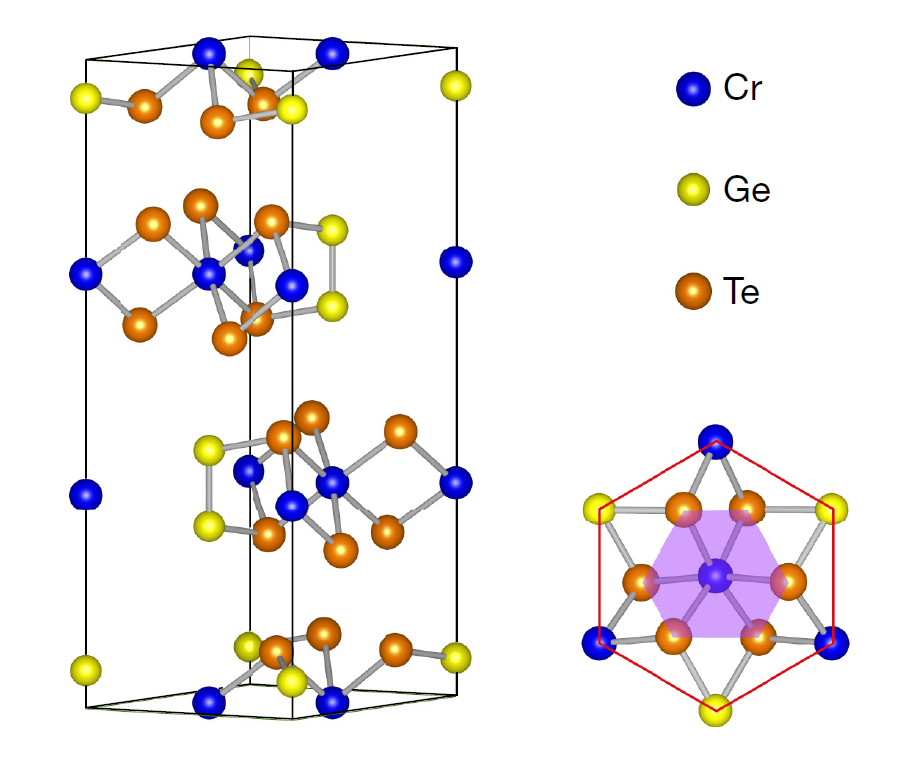
\includegraphics[width=0.45\textwidth]{fi_cgt_crystal}
	\caption{Crystal structure of \cgt{}.\\
		Source: Gong \etal{}, Nature Vol. 546, 265 (2017)}		
	\label{fig:fi_cgt_crystal}
	%	\vspace{-1.2cm}
	\vspace{-1cm}
\end{wrapfigure}

In this section, I will discuss various ferromagnetic insulator (FI) materials that might be used to stack with \bismuthselinide{}. Properties that will matter will include the cleanness of the interface, the lattice parameters, any resulting strain that might occur, and magnetic properties such as magnetisation amplitude. 
%TODO Cover 3D ferromagnetic insulators.
%I will cover a couple 3D ferromagnetic insulators that have been used in previous spin-torque heterostructure experiments, before detailing some newer few-layer 2D ferromagnetic insulators. 
I will cover new few-layer 2D ferromagnetic insulators that have potential to be used for spin-torque experiments.

FIs are rare, because most magnetic materials that incorporate iron, cobalt or nickel are often conductive. That being said, some 3D FIs have been known for a while, and recently some new FIs that can be exfoliated down to thin flakes have been discovered.

%\subsection{3D FIs}
%\subsubsection{BaFe$_{12}$O$_{19}$ (BFO)}
%BFO can be prepared by ALD, and can be grown to less than 5nm \cite{li_magnetization_2019}. 
%
%\subsubsection{Y$_3$Fe$_5$O$_{12}$ (YIG)}  is also a bulk film that can be grown thinly, for example down to 30nm in Wang \etal{} \cite{wang_surface-state-dominated_2016}.

\subsection{2D FIs}
\subsubsection{Chromium triiodide (CrI$_3$)} 

\begin{figure}[t]
	\centering
	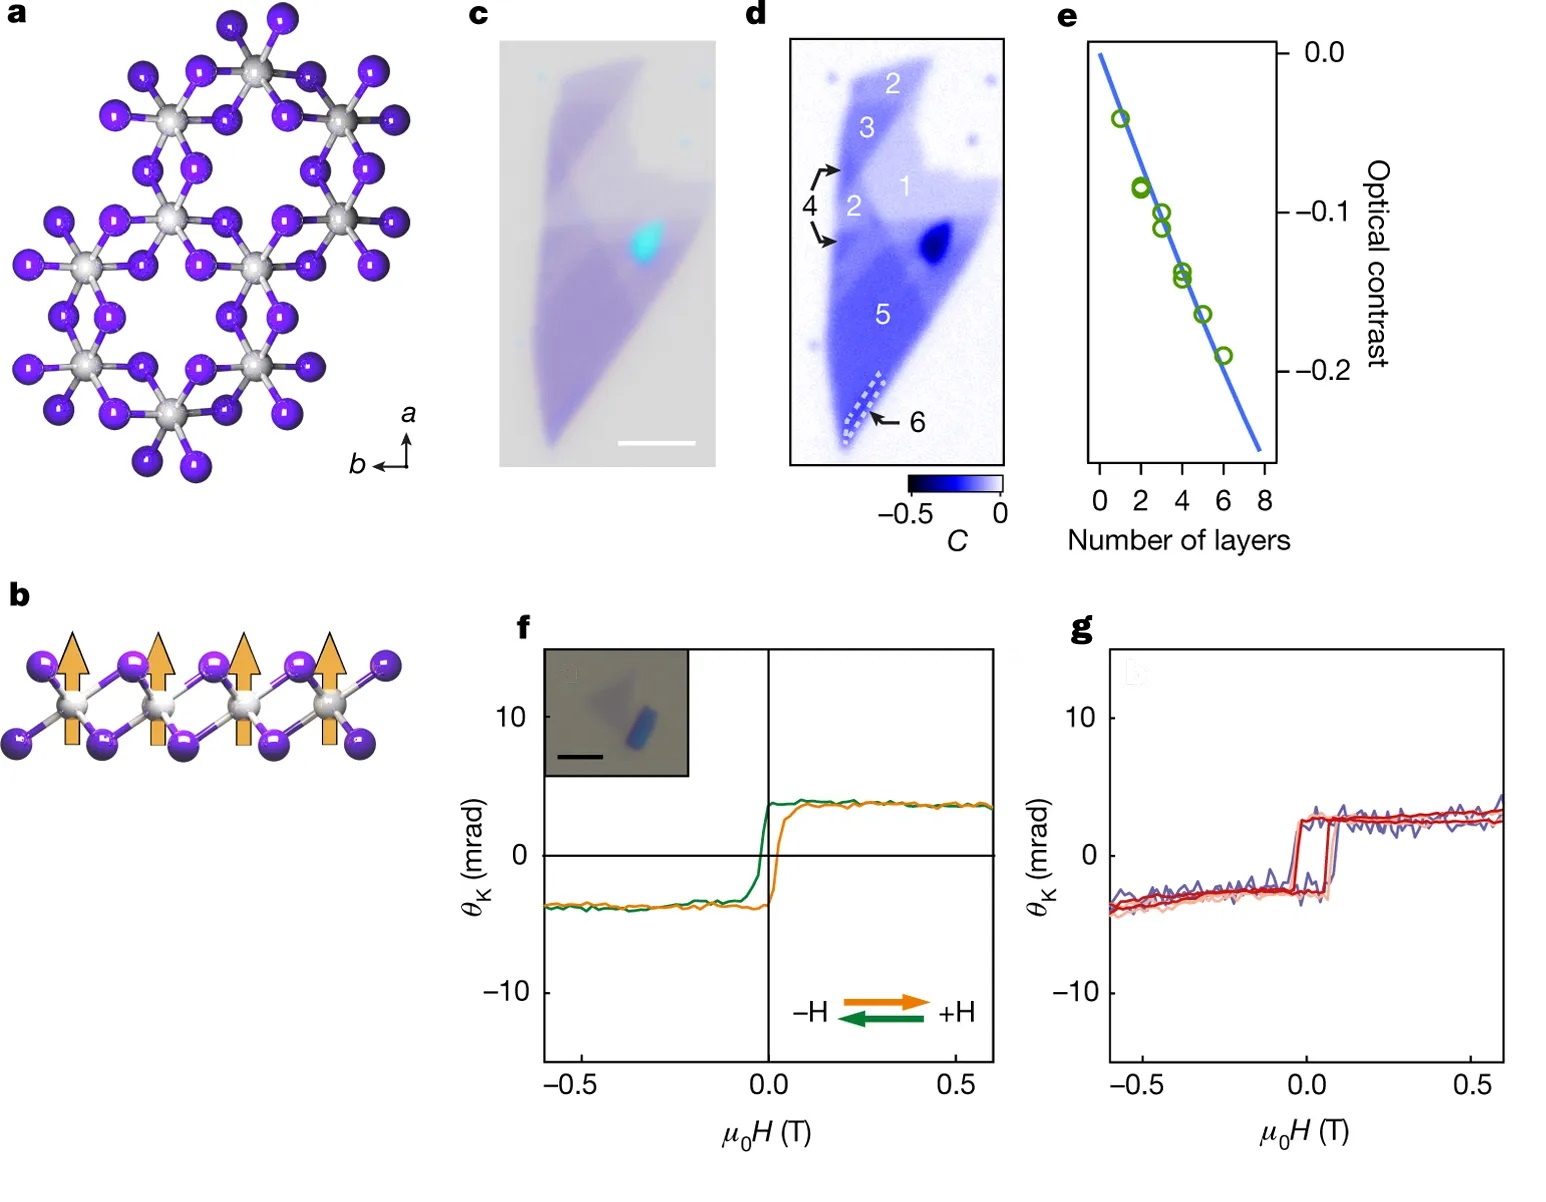
\includegraphics[width=0.8\textwidth]{fi_cri3_monolayer}
	\caption{\textbf{a)} \chromiumtriiodide{} monolayer atomic lattice. \textbf{b)} Out-of-plane view, depicting Ising spin. \textbf{c)} Optical image, scalebar 3$\mu$m. \textbf{d)} Calcualted contrast \textbf{e)} Linearity of contrast to thickness. \textbf{f)} Kerr signal of monolayer. \textbf{g)} Power dependence of Kerr signal taken at powers of 3 $\mu$W (blue), 10 $\mu$W (pink), 30 $\mu$W (red)\\
		Adapted from: Huang \etal{}, Nature Vol. 546, 270 (2017)}
	\label{fig:fi_cri3_monolayer}
\end{figure}

\chromiumtriiodide{} was first reported on around 2014 \cite{mcguire_coupling_2015}. The crystal undergoes a phase change below 220 K from monoclinic to rhombohedral. It has a Curie temperature at 61K in the bulk, and has a resistivity of 900 $\Omega$cm.

Recent reports have demonstrated \chromiumtriiodide{}'s ferromagnetic properties persist down to few-layers \cite{huang_layer-dependent_2017, huang_electrical_2018-1}. Huang \etal{} reports a curie temperature of 45K for monolayer \chromiumtriiodide{}, data shown in Fig. \ref{fig:fi_cri3_monolayer}. The followup paper shows electrostatic gate control of \chromiumtriiodide{} between ferromagnetic and anti-ferromagnetic states with some spin-locking \cite{huang_electrical_2018}. 

\subsubsection{\cgt{} (CGT)}
\cgt{} is also a new thin ferromagnetic insulator. It consists of quintuble layers, similar to \bismuthtelluride{} or \bismuthselinide{}, and is also terminated with hexagonal Te planes (Fig. \ref{fig:fi_cgt_crystal}), making it a van der Waals material. 

Crystals have been synthesised in bulk before through a flux method, such as demonstrated by Zhang \etal{} \cite{zhang_magnetic_2016}, with clear insulating and magnetic properties.

The discovery paper of 2017 \cite{gong_discovery_2017} shows that bilayers are stable for exfoliation, and magnetic order is found using a scanning Kerr microscope. It was noted that monolayers were thought to be invisible. Whilst the bulk material has a Curie temperature of 61K, the 2D material is less stable, being well defined below 40K. This is very similar to \chromiumtriiodide{}. While this is quite novel for investigating low dimensional physics and magnetic-spin effects, this material lacks the high temperature range to be practical around ambient temperatures. 

\begin{figure}[t]
	\centering
	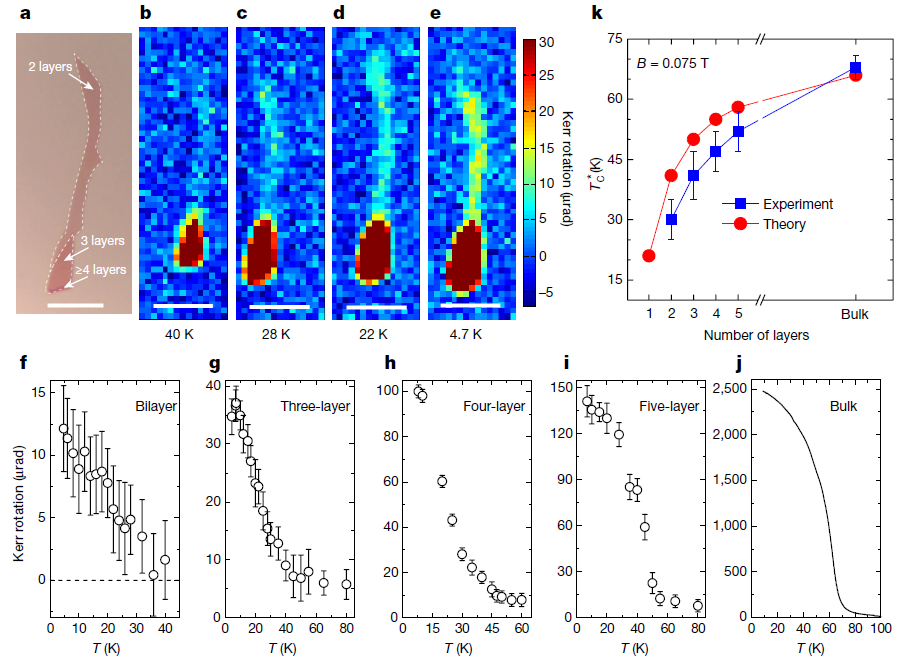
\includegraphics[width=0.8\textwidth]{fi_cgt_mag}
	\caption{\textbf{a)} Microscopy of \cgt{}. \textbf{b-e)} Appearance of Kerr rotation signal \textbf{f-j)} Temperature dependence of Kerr signal in different thicknesses. \textbf{k)} Calculations of transition temperatures.\\
		Source: Gong \etal{}, Nature Vol. 546, 265 (2017)}
	\label{fig:fi_cgt_mag}
\end{figure}

More recent transport data was published by using Pt electrodes, showing the conductivity that appears above 60 K, compared to the massive resistance below\cite{lohmann_probing_2019}. There are also promising predictions to increase the Curie Temperature of CGT towards liquid nitrogen temperatures, through the use of absorption of gas molecules (NO, NO$_2$) \cite{he_remarkably_2019}. 

The perpendicular magnetic anisotropy (PMA) is a measure of how strong the magnetic interactions are in the perpendicular direction. This is particularly important for memory or torque devices. For CGT, a PMA energy of $10^5$ erg/cm$^3$ is reported \cite{zhang_van_2019}.

\subsubsection{Magnesium Titinate (MgTiO$_3$, MTO)}
MTO is another recent addition to thin film ferromagnetic insulator films. Frantti \etal{} reported the stoichiometric material in 2019\cite{frantti_quest_2019}. 

\begin{figure}[t]
	\centering
	\begin{minipage}[t]{.95\textwidth}
		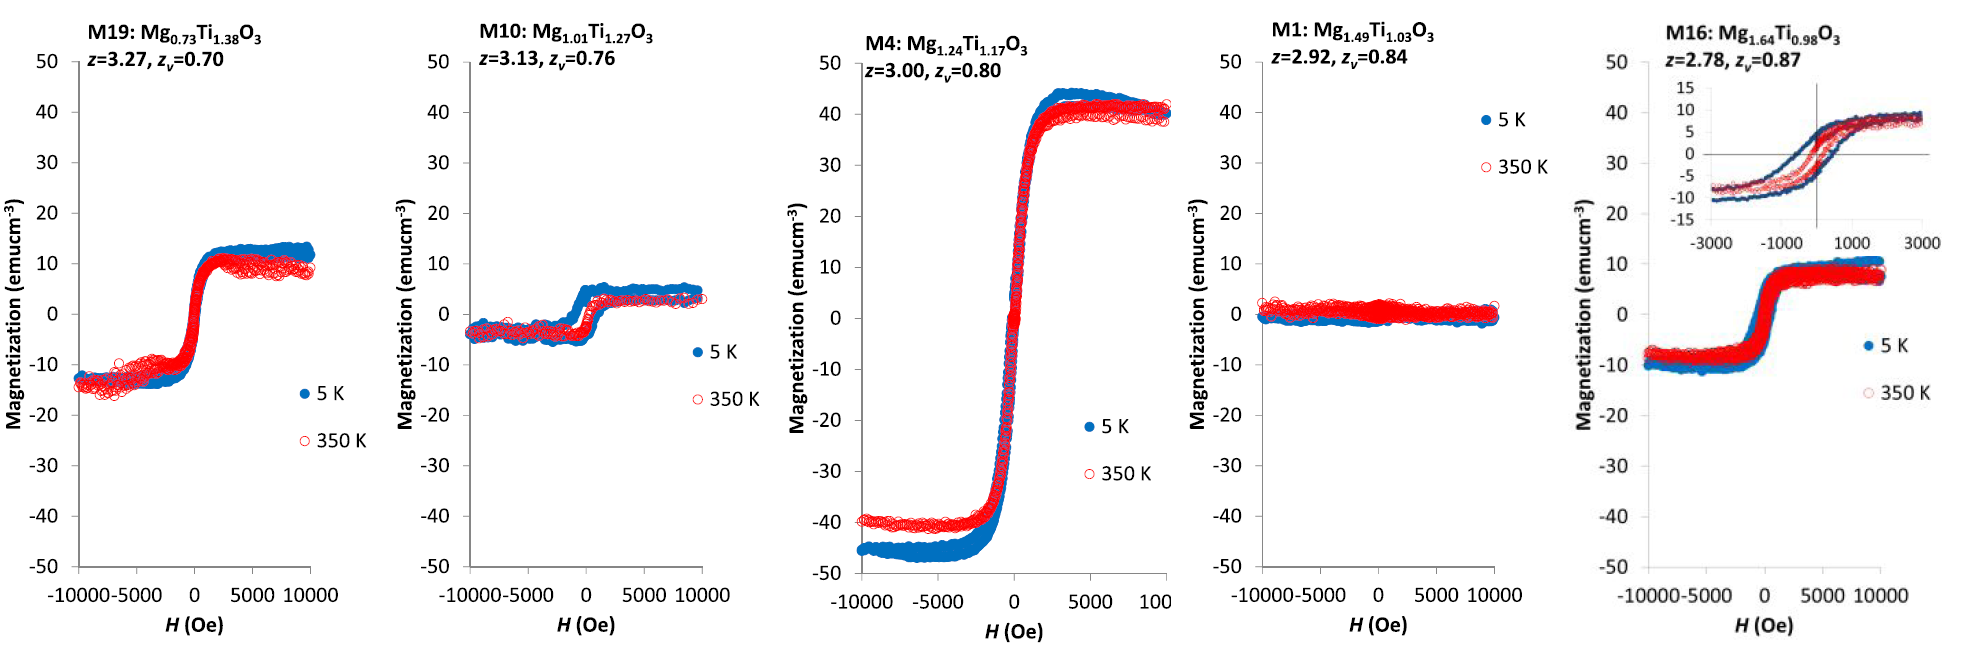
\includegraphics[width=\linewidth]{fi_mgo_magn}
		\caption{Magnetisation measurements for various mixtures of Mg and Ti in MGO, for two different temperatures. Average valence $z$ and octahedral filling fractions $z_v$ are shown.\\
		Source: Frantti \etal{}, J. Phys. Chem. C 123, 19970 (2019)}		
		\label{fig:fi_mgo_magn}
	\end{minipage}
\end{figure}

MTO has a rhombohedral ilmenite structure, and in this study was grown via a pulsed lazer deposition technique to deposit films of thicknesses around 50-60 nm. Across a variety of samples, Frantti saw magnetization swings of up to $\Delta M = 80$ emu cm$^{-3}$ $= 8 \times 10^4$ Am$^{-1}$ (see Fig. \ref{fig:fi_mgo_magn}). A few resistivity measurements of samples were reported, which were $0.07$ and 265 M$\Omega$ cm, the latter reported to be very typical of most samples.

%\subsection{2D Ferromagnetic Conductors}

\subsubsection{Other 2D ferromagnetic materials}
While an insulator is preferable due to the clear picture expected when interfacing with topological insulator surface states, it's worth noting other 2D ferromagnetic developments. As of 2018, Fe$_3$GeTe$_2$ has also been recognised as a 2D van der Waals material possessing ferromagnetism to a much higher Curie temperature ($\sim 230$ K) \cite{deng_gate-tunable_2018}. This material also has a much larger PMA than CGT, boasting $\sim 10^7$ erg/cm$^3$.

%\textcolor{red}{Todo: discuss lattice matching in heterostructures page?}
%TODO: Discuss lattice matching.